\section{Kinematics of a particle}

\label{sec:particle}

Let us focus again on a fluid particle, as we did on Sections
\ref{sec:continuity} and \ref{sec:pressure_forces}, but now focusing
on how the particle itself distorts as a consequence of a velocity
field.

All possible distortions of a particle will be a combination of the
following:
\begin{enumerate}
 \item Translation
 \item Rotation
 \item Shear
 \item Dilation
\end{enumerate}

A translation is just the motion of its center of mass from one place
to another, and for a small time is given simply by $\bfu dt$. The
other motions are more complicated, since they involve spatial
derivatives of the velocity. They must: for a constant velocity field
translation is the only motion that occurs.

\subsection{Rotation}

We will refer to particle in figure \ref{fig:}, with vertices A, B,
and C. Vertex D plays no role --- also, it is sufficient to focus on
the face that is portrait, even if the shape of a particle is supposed
to be a cube. It is straightforward to include the other faces, as we
will see.

After a small time $d$ the particle has distorted, so that the
vertices are now at positions A', B', C', and D'.

\begin{figure}
  \centering
  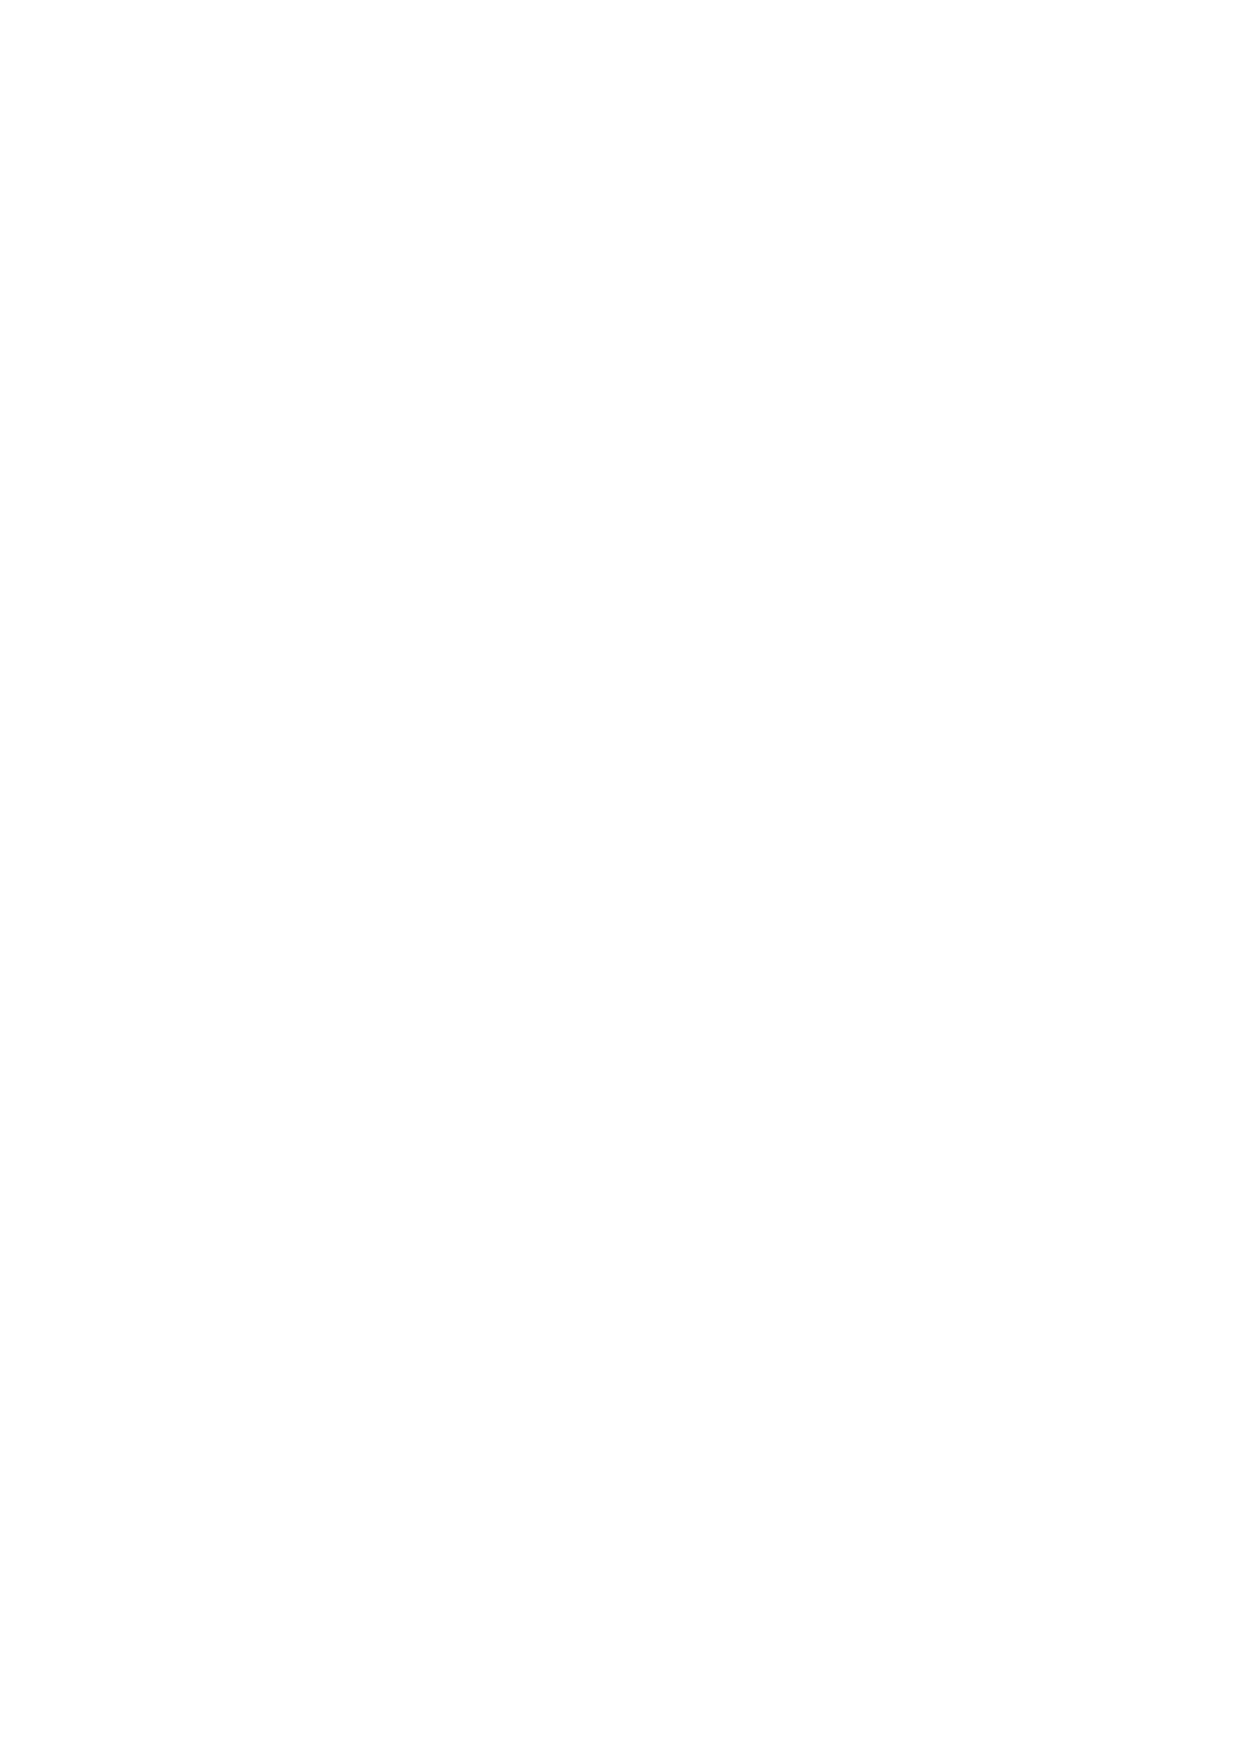
\includegraphics[width=0.4\linewidth]{figures/particle0}
  \caption{\label{fig:particle0}}
\end{figure}



Let us call $\alpha$ the angle between the $x$ axis and the A'-B'
edge, with the usual counter-clockwise convention as
positive. Similarly, $\beta$ is the angle between the A'-C' edge and
the $y$ axis, with the same convention. It is obvious that a net
rotation takes place if e.g. both angles are positive. If, on the
other hand, they are equal in magnitude but differ in sign, no
rotation takes place. This makes it reasonable to define the
rotation as the average of both angles:
\[
d\Omega_z = \frac12
\left(
        \alpha + \beta
\right) .
\]

Now, angle $\alpha$ will always be very small as $dt$ gets very
tiny. Hence, we may approximate it by its tangent:
\[
\alpha \approx \frac{d\ell}{dx'}
\]



\begin{figure}
  \centering
  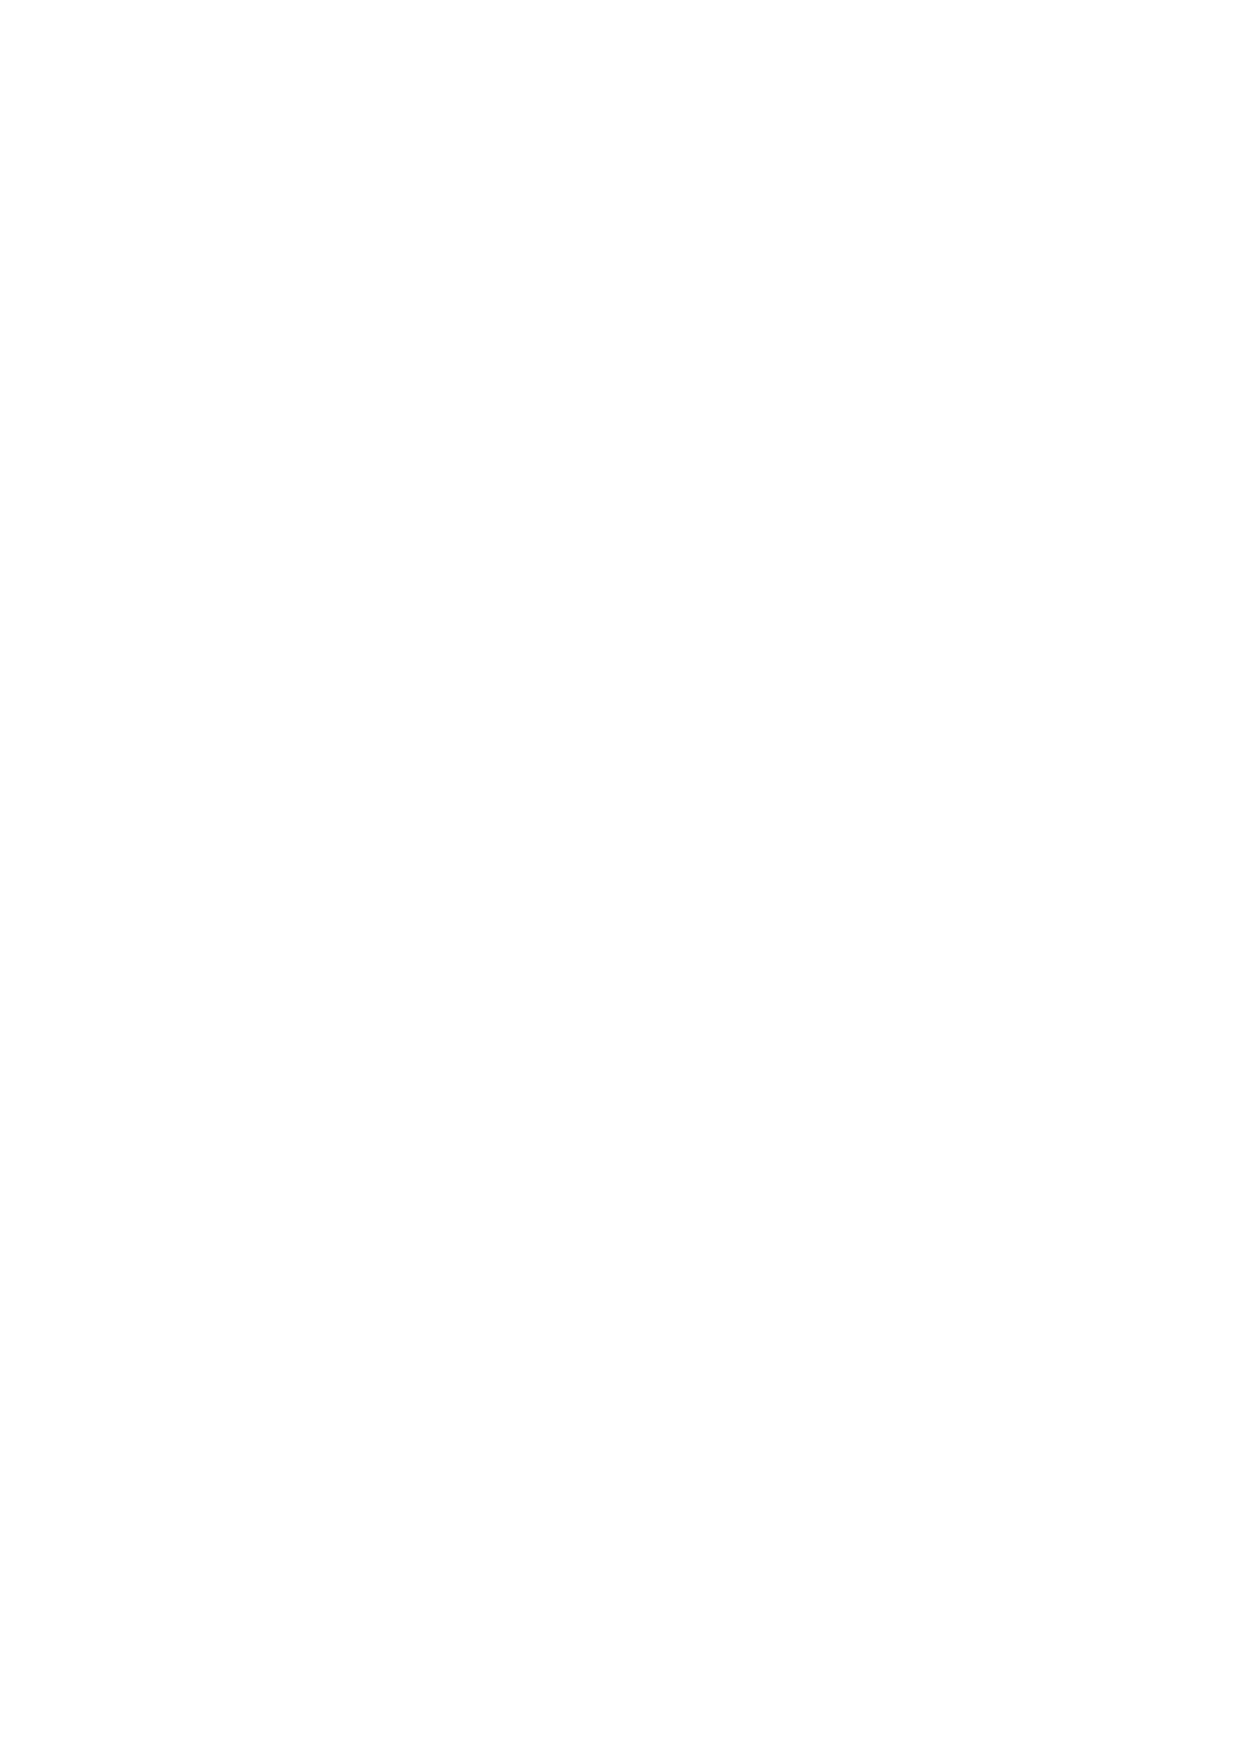
\includegraphics[width=0.4\linewidth]{figures/particle1}
  \caption{\label{fig:particle1}}
\end{figure}

For a small time interval, we have the following:
\begin{align*}
	dx' & =
	  x(B')-x(A') \approx
	 (dx+v_x(B) dt) - v_x(A) dt  \\
	& \approx
	dx+
	\left(
	v_x(A) +
	\frac{\partial v_x}{\partial x} dx
	\right ) dt - v_x(A) dt \\
	& = dx + \frac{\partial v_x}{\partial x} dx dt ,
\end{align*}
where we have taken the origin to coincide with the position of A. The
partial derivative is supposed to be evaluated at A, but in the limit
as $dx$ goes to zero it is just ``at the particle''. Similarly, the opposing
side is:
%
\begin{align*}
d\ell & = y(B')-y(A') \approx
y(B) + 
v_y(B) dt
-
y(A) - 
v_y(A) dt \\
& =
\left(
v_y(B) - v_y(A) 
\right) dt 
 \approx
\frac{\partial v_y}{\partial x} dx dt
.
\end{align*}
%
Therefore, to first order in $dt$:
\[
\alpha \approx \frac{\partial v_y}{\partial x}  dt .
\]
In other words, the rate of change of the angle is
\[
\frac{d \alpha}{dt} = \frac{\partial v_y}{\partial x}  .
\]
Notice the cross derivative: what is relevant is the change of the
vertical component of the velocity with the horizontal coordinate.

A similar calculation for the other angle reveals
\[
\frac{d \beta}{dt} = - \frac{\partial v_x}{\partial y}  .
\]

Taking all
\[
\frac{d\Omega_z}{dt} = \frac12
\left(
  \frac{\partial v_y}{\partial x}  -
  \frac{\partial v_x}{\partial y}
\right) .
\]

This may sound familiar to the reader, since the curl in Cartesian
coordinates has a $z$ component with exactly the same expression, but
the factor of $1/2$. This analysis may be carried out for
rotations about the other two Cartesian axes, with the end result that
\[
 \frac{d \bm{\Omega} }{dt} = \frac12 \vort .
\]

The curl is therefore twice the rate of rotation of a fluid particle.


As an example, let us consider a uniform circular motion about the
origin:
\[
\bfr =
\begin{cases}
x =r \cos(\omega_0 t) \\
y =r \sin(\omega_0 t) .
\end{cases}
\]
The velocity field is
\[
\bfu =
\begin{cases}
u_x= -r \omega_0 \sin(\omega_0 t) = -\omega_0 y \\
u_y=  r \omega_0 \cos(\omega_0 t) =  \omega_0 x.
\end{cases}
\]

If we compute the curl of this field, its only component is the $z$ one:
\[
\omega_z= \left(
  \frac{\partial (\omega_0  x)}{\partial x}  -
  \frac{\partial (- \omega_0 y) }{\partial y}
\right) =  2 \omega_0 . 
\]

Therefore, the curl indeed is twice the angular velocity.

Finally, let us recall, from the definition of the tensor
$\nabla \bfu$ of Eq. \ref{eq:nabla_u_def},
\begin{equation}
  \label{eq:dOmega_as_grad_u}
  \frac{d\Omega_{ij}}{dt} = \frac12
  \left[
    (\nabla \bfu)_{ij} -
    (\nabla \bfu)_{ji}
  \right] ,  
\end{equation}
%
where the cyclic convention $(i,j,k)$ is implied in order to relate
the indices of $d\Omega_{ij}/ dt$ and the components $d\Omega_k/ dt$
(see Exercise \ref{ex:dOmega_LC} for a definition in terms of the
Levi-Civita symbol.)


\subsection{Strain}

Similarly to the definition of rotation, let us define the strain as
half the difference between angle $\beta$ and $\alpha$:
\[
d\epsilon_{xy} = \frac12
\left(
        \alpha - \beta
\right) .
\]
Indeed, if both are equal we get a pure rotation, and no strain. If,
however, they have the same magnitude but opposite sign, we have a pure
strain and no rotation.

This definition leads to the rate of strain tensor
\[
\epsilon_{xy} = \frac12
\left(
  \frac{\partial v_y}{\partial x}  +
  \frac{\partial v_x}{\partial y}
\right) .
\]

Notice the notation: indices $xy$ implay a strain on that plane. In general,
\[
\epsilon_{ij} = \frac12
\left(
  \frac{\partial v_j}{\partial x_i}  +
  \frac{\partial v_i}{\partial x_j}
\right) .
\]

This defines off-diagonal terms of a tensor that is obviously
symmetric. All together, three terms in 3D ($xy$, $xz$, and $yz$).

Also, from the definition of the tensor $\nabla \bfu$ of
Eq. \ref{eq:nabla_u_def},
\begin{equation}
  \label{eq:epsilon_as_grad_u}
  \epsilon_{ij} = \frac12
  \left[
    (\nabla \bfu)_{ij} +
    (\nabla \bfu)_{ji}
  \right] ,
\end{equation}
so that $\epsilon$ is the symmetrized version of the gradient of the
velocity. In compact notation,
\begin{equation}
	\label{eq:epsilon_as_grad_u_compact}
	\epsilon = \frac12
	\left[
	\nabla \bfu +
	\nabla \bfu^{\tran}
	\right] .
\end{equation}


We may also extend these definitions to the diagonal terms:
\[
  \epsilon_{ii} =   \frac{\partial v_i}{\partial x_i} ,
\]
which are not really strains, as we show next.

\subsection{Dilation (or compression)}

We have derived before that the change on side $dx$ is
\[
dx' \approx  dx + \frac{\partial v_x}{\partial x} dx dt ,
\]
which features the diagonal components of the strain tensor just
introduced. In general, for the $i$ Cartesian direction,
\[
dx_i' \approx dx_i + \epsilon_{ii} dx_i dt = dx_i
\left(
1+\epsilon_{ii} dt
\right)
\]

If we consider the volume, its new value will be
\[
V'= dx' dy' dz'  \approx  \prod_i  dx_i \left( 1+\epsilon_{ii} dt \right)
\approx \left(\prod_i  dx_i \right) \left( 1 + \sum_j  \epsilon_{jj} dt \right) ,
\]
where in the last expression we have neglected all higher order terms
($dt^2$ or higher). Therefore, the new volume of a particle is
\[
V' = V \left( 1 + \sum_j  \epsilon_{jj} dt \right) .
\]
Its change is
\[
V'-V =  V \sum_j  \epsilon_{jj} dt .
\]
In the limit as $dt\to 0$,
\[
\frac{d V}{dt} = V \sum_j  \epsilon_{jj} .
\]
This clearly identifies the diagonal components of the strain rate tensor
as those responsible for the relative rate of change of the volume.
Moreover, due to its definition, the sum of all components (i.e. the
trace of the tensor) is precisely the divergence of the velocity:
\[
\sum_j  \epsilon_{jj} = \nabla\cdot \bfu .
\]

We therefore arrive at the expression for the rate of change of a particle:
\[
\frac{d V}{dt} = V  \nabla\cdot \bfu .
\]

Also, and since the diagonal terms of the rate of strain tensor are
not really related to strain at all, there is the possibility to subtract them
to build what is called the deviatoric \index{deviatoric} rate of strain tensor:
\[
\tilde{\epsilon}_{ij} := \epsilon_{ij} - \frac13 \epsilon_{kk} \delta_{ij} .
\]
The tensor is traceless by construction. In compact notation,
\begin{equation}\label{eq:deviatoric_rate_of_strain}
	\tilde{\epsilon} := \epsilon - \frac13 \left( \nabla\cdot \bfu \right)  \eye =
\frac12
\left[
\nabla \bfu +
\nabla \bfu\tran
\right] - \frac13 \left( \nabla\cdot \bfu \right)  \eye .
\end{equation}


Is is easily demonstrated, that the tensor is traceless, since
$\Tr  \nabla\bfu = \Tr \nabla\bfu\tran = \divu $. Therefore,
\[
\Tr \left( \frac12 \nabla\bfu + \frac12 \nabla\bfu\tran -\frac13 (\divu) \eye \right) =
2\times \frac12 \divu - 3\times \frac13 (\divu) = 0 .
\]




\subsection{Continuity, re-revisited}
\label{sec:continuity3}

This is the expression that was lacking in our derivation in
Section \ref{sec:continuity}. Indeed, if the mass of a particle is
constant, it is trivial to recover the continuity equation for the
density. The latter is $\rho=m/V$, therefore,
\[
\frac{d \rho }{dt} =
\frac{d (m/V) }{dt} = \frac1V \underbrace{\frac{ dm }{dt}}_{=0} -
m\frac1{V^2}  \frac{ dV }{dt } =
- m\frac1{V}  \nabla\cdot \bfu  = -\rho \nabla\cdot \bfu ,
\]
which indeed is the right expression (the ``convergence'' Equation
\ref{eq:convergence}.)

This also shows that we are working on an Lagrangian reference frame, so
that advective derivatives appear naturally. Indeed, $dm/dt=0$ for a
particle, whereas mass may enter and leave a fixed (Eulerian) zone in
space.

